\section{Identities}

\subsection{Periodicity}
From both the definition of trigonometric functions, and their graphs, we can see that they are inherently {\bf periodic functions}.  As the angle of rotation increases without limit, every trigonometric function repeats itself.  The number of rotations are irrelevant to sine and cosine;  they depend only on the final rotational position.  Because one complete rotation of an angle is $2\pi$ radians, we can deduce that the {\bf period} of these functions is $2\pi$.  That is,\\

\tab$sin(\theta) = sin(\theta \pm 2\pi n), \ \ n=0,1,2,...$\\

\tab$cos(\theta) = sin(\theta \pm 2\pi n), \ \ n=0,1,2,...$\\

From these, we can derive that the tangent, cotangent, secant, and cosecant also periodic.

\begin{figure}[htb]
\center
\caption{Periodicity of trig. functions.}
\label{fig:preiodicity of trig. functions}
\begin{tikzpicture}[inner sep=0pt,minimum size=0mm]

\node at (0,5){};

\node at (22.5:4.25) {$\frac{\pi}{4}$};
\node at (22.5:3.35) {$\frac{9\pi}{4}$};
\node at (22.5:2.1) {$\frac{17\pi}{4}$};

\AXES{0}{0}{4}{3.5}
\LANGLE{0,0}{4}{0}{45}{}
\SPIRAL{0}{45+360}{3.05}{2.8}{}
\SPIRAL{0}{45+360+360}{1.75}{1.25}{}

\node at (-0.35,2) {$sin$};
\draw[dotted] (0,4*0.7071) -- (4*0.7071,4*0.7071);
\draw[very thick,->] (0,0) -- (0,4*0.7071);

\node at (2,-0.35) {$cos$};
\draw[dotted] (4*0.7071,0) -- (4*0.7071,4*0.7071);
\draw[very thick,->] (0,0) -- (4*0.7071,0);

\end{tikzpicture}
\end{figure}


\subsection{Negative Angles}

We can graphically show how trigonometric functions respond to negative angles.  For a negative angle, the y projection of the angle is negated, while the x projection is not.  Thus,\\

\tab$sin(-\theta) = - sin(\theta)$\\

\tab$cos(-\theta) = cos(\theta)$\\

Another way to describe this is by calling sine an {\bf odd function}, and cosine an {\bf even function}.  The definition of an odd function is $f(-x) = -f(x)$, and the definition of an even function is $f(-x)=f(x)$.  Graphically, an even function is symmetric about the y axis, and an odd function has rotational symmetry about the origin.  Keep in mind that a function may be neither even nor odd.\\

\begin{figure}[htb]
\center
\caption{Negative angles and trig. functions.}
\label{fig:negative angles and trig. functions}
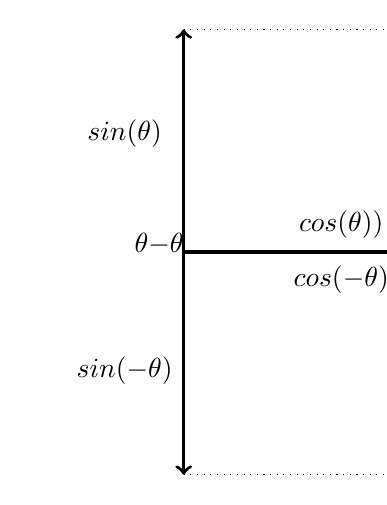
\begin{tikzpicture}[inner sep=0pt,minimum size=0mm]

\PXAXES{0}{0}{4}{3.25}
\LANGLE{0,0}{4}{0}{45}{$\theta$}
\LANGLE{0,0}{4}{0}{-45}{$-\theta$}

\node at (-0.75,1.5) {$sin(\theta)$};
\draw[dotted] (0,4*0.7071) -- (4*0.7071,4*0.7071);
\draw[very thick,->] (0,0) -- (0,4*0.7071);

\node at (-0.75,-1.5) {$sin(-\theta)$};
\draw[dotted] (0,-4*0.7071) -- (4*0.7071,-4*0.7071);
\draw[very thick,->] (0,0) -- (0,-4*0.7071);


\node at (2,0.35) {$cos(\theta))$};
\node at (2,-0.35) {$cos(-\theta)$};
\draw[dotted] (4*0.7071,0) -- (4*0.7071,4*0.7071);
\draw[dotted] (4*0.7071,0) -- (4*0.7071,-4*0.7071);
\draw[very thick,->] (0,0) -- (4*0.7071,0);

\end{tikzpicture}
\end{figure}

By referring to the graphs in the previous chapter, we can see that the secant is an even function, and the cosecant, tangent, and cotangent are odd functions.\\

\subsection{Rearrangements}

From the definitions of the standard trigonomtetric functions, we can derive many simple relationships. \\

\tab$tan(\theta) = \frac{sin(\theta)}{\cos(\theta)} = sin(\theta)sec(\theta)$\\

\tab$cot(\theta) = \frac{cos(\theta)}{\sin(\theta)} = cos(\theta)csc(\theta)$\\

\tab$cos(\theta)tan(\theta)=sin(\theta)$\\

\tab$sin(\theta)cot(\theta)=cos(\theta)$\\

It is often recommended to memorize many of these simple rearrangements of trigonometric identities, but not necessary, as any combination of trigonometric functions can be rewritten in terms of sine and cosine, and then simplified.\\

\subsection{The Pythagorean Identity}

Let us look at a rotation by an angle theta of a line with length $r$, and the resulting projections $x$ and $y$.\\

\begin{figure}[htb]
\center
\caption{Angle and projections.}
\label{fig:angle and projections}
\begin{tikzpicture}[inner sep=0pt,minimum size=0mm]
\node at (0,3.5) {};

\PAXES{0}{0}{4.5}{2.5}
\LANGLE{0,0}{4}{0}{30}{$\theta$}

\node at (1.5,1.25) {$r$};

\node at (-0.25,1) {$y$};
\draw[dashed] (0,4*0.5) -- (4*0.866,4*0.5);
\draw[very thick,->] (0,0) -- (0,4*0.5);

\node at (1.75,-0.25) {$x$};
\draw[dashed] (4*0.866,0) -- (4*0.866,4*0.5);
\draw[very thick,->] (0,0) -- (4*0.866,0);


\end{tikzpicture}
\end{figure}


By the Pythagorean Theorem (or the Cartesean distance formula), we can see that \\

\tab$x^2 + y^2 = r^2$\\

\tab$\implies \frac{x^2}{r^2} + \frac{y^2}{r^2} = 1$\\

\tab$\implies (\frac{x}{r})^2 + (\frac{y}{r})^2 = 1$\\

We can substitute the definition of sine and cosine into this equation, to yield\\

\tab$sin(\theta) = \frac{y}{r}, \ \ cos(\theta) = \frac{x}{r}$\\

\tab$\implies sin^2(\theta) + cos^2(\theta) = 1$\\

This is known as the {\bf Pythagorean Identity}.  It shows the fundamental relationship between the sine and cosine of an angle.\\

Through rearrangement, we can derive other equivalent pythagoren identities, but again, these need not be memorized.\\

\tab$sin^2(\theta) + cos^2(\theta) = 1$\\

\tab$\implies \frac{sin^2(\theta)}{cos^2(\theta)} + \frac{cos^2(\theta)}{cos^2(\theta)} = \frac{1}{cos^2(\theta)}$\\

\tab$\implies tan^2(\theta) + 1 = sec^2(\theta)$\\

Or,\\

\tab$sin^2(\theta) + cos^2(\theta) = 1$\\

\tab$\implies \frac{sin^2(\theta)}{sin^2(\theta)} + \frac{cos^2(\theta)}{sin^2(\theta)} = \frac{1}{sin^2(\theta)}$\\

\tab$\implies 1 + cot^2(\theta) = csc^2(\theta)$\\

\subsection{Review}

\begin{enumerate}

\item{Find 3 equivalent angles for each of the following:\\

\tab a) $30^o$\\

\tab b) $\frac{7\pi}{6}^c$\\

\tab c) $115^o$\\

\tab d) $\frac{-\pi}{2}$\\

\tab e) $0^o$\\}

\item{Write whether each of the following trig. functions are even, odd, or neither, and prove it:\\

\tab a) $tan(\theta)$\\

\tab b) $cot(\theta)$\\

\tab c) $sec(\theta)$\\

\tab d) $csc(\theta)$\\

\tab e) $sin(\theta) - cos(\theta)$\\}

\item{Simplify the following expressions:\\

\tab a) $cos^2(\theta)tan(\theta)$\\

\tab b) $csc(\theta) - cos(\theta)cot(\theta)$\\

\tab c) $1 + cot^2(\theta)$\\

\tab d) $\frac{sin^2(\theta)tan^2(\theta) + sin^2(\theta)}{tan^2(\theta)}$\\

\tab e) $\frac{(sec(\theta) + tan(\theta))(sec(\theta) - tan(\theta))}{(csc(\theta) - cot(\theta))(csc(\theta) + cot(\theta))}$\\}

\item{Given that the sine of an angle is 0.73, what is the cosine?  the tangent?\\}

\item{Given that the tangent of an angle is 0.5 and the angle is in the first quadrant, what is the cosine?}

\end{enumerate}

